\chapter{描述运动：轨迹与速度}\label{ch:g6:describing-motion}

飘落的树叶、高速列车、旋转木马上的木马、
一记点球：世界从不静止。为研究运动，物理学对每个运动的物体提出
两个简明的问题：\emph{沿着什么路径？}
和\emph{沿路径\omterm{def:g5:speed-distance-time:speed}{速度}多快？}路径与快慢——\omterm{def:g6:describing-motion:trajectory}{轨迹}与
\omterm{def:g5:speed-distance-time:speed}{速度}——正是本章的一对“眼镜”。

\section{轨迹：所经的路径}

\begin{definition}[轨迹]\label{def:g6:describing-motion:trajectory}
运动物体的\emph{轨迹}\index{轨迹}是
物体运动时所描出的线——即它在空间中划出的路径。
日常生活中，轨迹大多可归为三种形状：
\emph{直线的}\index{直线轨迹}（电梯、
落下的苹果），\emph{圆周的}\index{圆周轨迹}（旋转木马上的木马、
钟表指针的尖端），以及更为自由的\emph{曲线的}形状（抛出的球的弧线、
燕子的俯冲）。
\end{definition}

\begin{omfigure}
\begin{tikzpicture}[scale=0.85]
  \draw[-Stealth, very thick, omDef] (0.8,0.3) -- (0.8,3.3);
  \fill[omExo] (0.8,0.3) circle (0.14);
  \node[below, font=\small] at (0.8,-0.1) {电梯：直线的};
  \draw[very thick, omDef] (4.7,1.8) circle (1.3);
  \fill[omExo] (6.0,1.8) circle (0.14);
  \draw[-Stealth, omDef, very thick] (6.0,1.95) -- (5.95,2.35);
  \node[below, font=\small] at (4.7,-0.1) {旋转木马：圆周的};
  \draw[-Stealth, very thick, omDef]
    (8.2,0.3) .. controls (9.2,3.6) and (10.6,3.6) .. (11.4,0.5);
  \fill[omExo] (8.2,0.3) circle (0.14);
  \node[below, font=\small] at (9.9,-0.1) {抛出的球：曲线的};
\end{tikzpicture}

{\small 三种常见\omterm{def:g6:describing-motion:trajectory}{轨迹}：直线上升、
无尽的圆周、抛出的弧线。}
\end{omfigure}

\begin{example}[谁的轨迹？]\label{ex:g6:describing-motion:whose}
注意说明所跟踪的是\emph{哪一个点}。旋转木马上木马的
鼻子画出一个圆；整个旋转木马的中心则
什么也不画——它始终静止。滚动车轮的轮毂沿直线
滑行，而轮缘上的一点则描出优美的跳跃状\omterm{def:g6:describing-motion:trajectory}{轨迹}。
一台机器，多条\omterm{def:g6:describing-motion:trajectory}{轨迹}：物理学每次只追踪一个点。
\end{example}

\begin{remark}[相对于什么而运动？]\label{rem:g6:describing-motion:relative}
坐在火车上打盹的乘客，相对于对面的乘客根本画不出任何\omterm{def:g6:describing-motion:trajectory}{轨迹}，
而田野上观望的牛却看到地图上一条长达一百千米的线。
两种描述都是正确的：运动总是\emph{相对于某物的运动}，
描述者必须说明参照的是什么。目前我们默认一切都相对于地面而言；
选择其他观察视角的完整威力，
是一个值得称道的精彩故事，留待
高中分册再讲。
\end{remark}

\begin{omfigure}
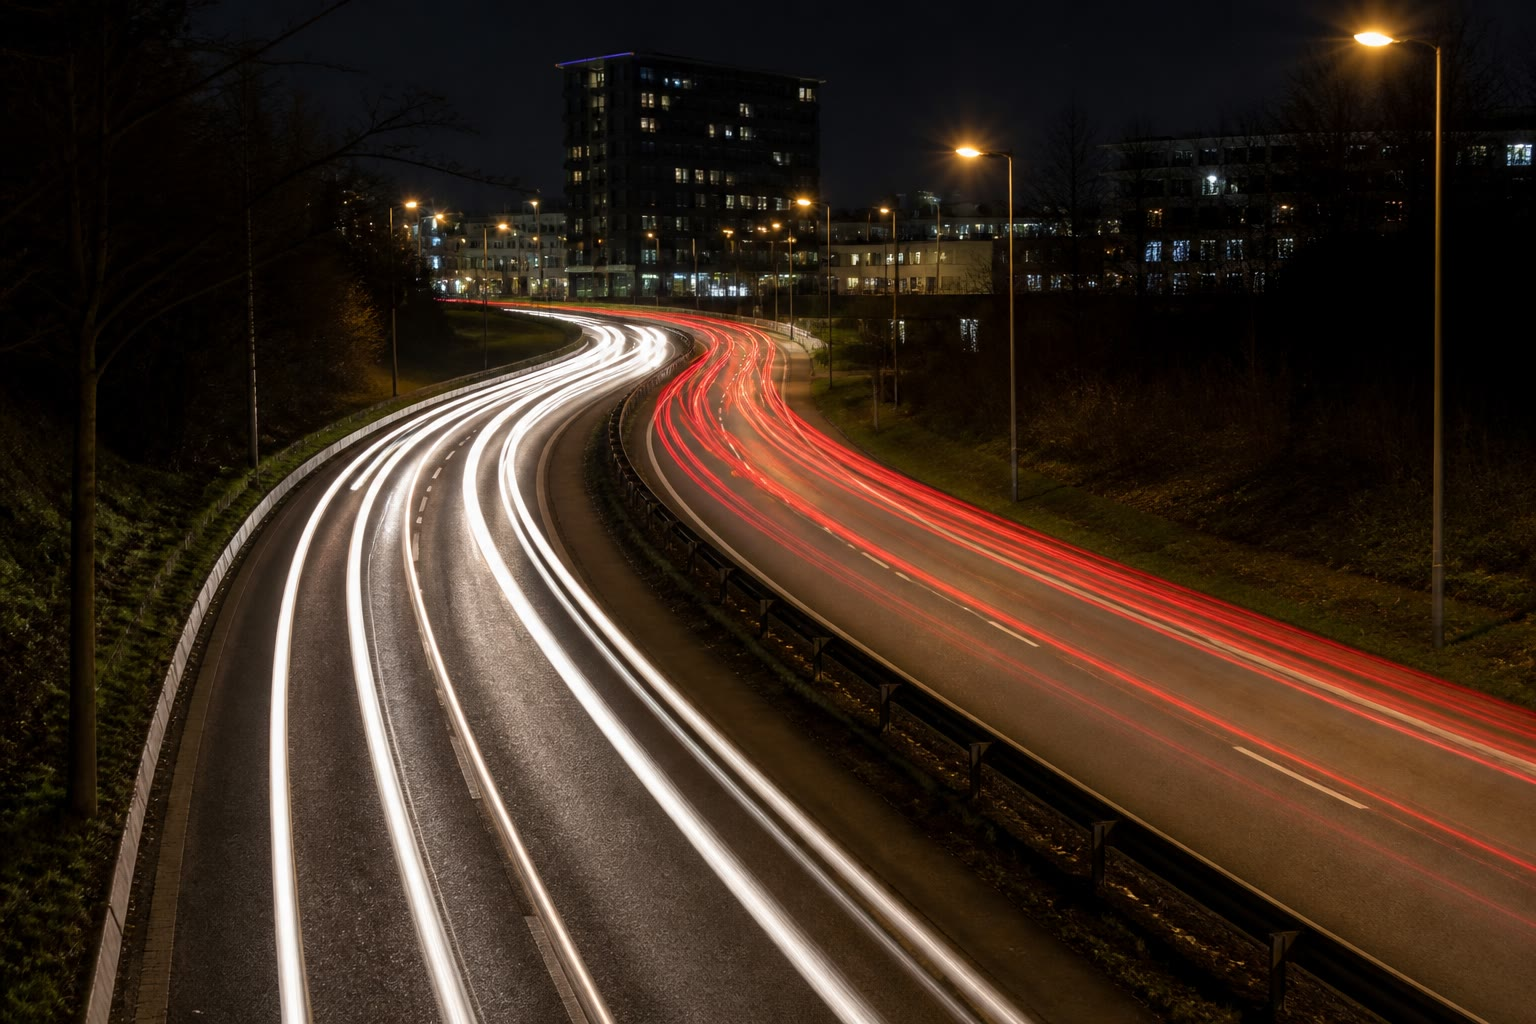
\includegraphics[width=0.55\linewidth]{images/book1/ai/g6-motion-light-trails.jpg}

{\small 夜间长时间开着快门的相机会拍出\omterm{def:g6:describing-motion:trajectory}{轨迹}：每一盏车灯都描出了其所属汽车所经过的确切路径。}
\end{omfigure}

\section{匀速还是变速？}

\begin{definition}[匀速运动与变速运动]\label{def:g6:describing-motion:uniform}
运动在相等的时间内通过相等的距离时，称为\emph{匀速运动}\index{匀速运动}，
例如按节拍器节奏平稳的步行、列车在两站之间的平稳行驶。
若\omterm{def:g5:speed-distance-time:speed}{速度}发生变化，则称为\emph{变速运动}\index{变速运动}：
加速（起跑后的短跑运动员）、
减速（刹车的公交车），
或二者交替出现（城市交通中无尽的走走停停）。
\end{definition}

\begin{proposition}[读懂点迹照片]\label{prop:g6:describing-motion:dots}
以相等的时间间隔为运动物体拍照——把许多快照叠在同一张图上——
运动便会在图中以点留下自己的“签名”，
其特征如下：
\begin{enumerate}
  \item 点间距均匀：\omterm{def:g6:describing-motion:uniform}{匀速运动}；
  \item 点间距沿途逐渐增大：加速；
  \item 点间距逐渐减小：减速。
\end{enumerate}
相邻两点之间的时间间隔都相等，因此点与点之间的间距
恰好反映了各段的距离——一眼便可作出判断。
\end{proposition}

\begin{omfigure}
\begin{tikzpicture}[scale=0.85]
  \foreach \x in {0.5,2.0,3.5,5.0,6.5,8.0,9.5} {
    \fill[omDef] (\x,2.6) circle (0.13);
  }
  \node[right, font=\small] at (10.1,2.6) {匀速的};
  \foreach \x in {0.5,1.1,1.9,3.0,4.4,6.1,8.1} {
    \fill[omThm] (\x,1.5) circle (0.13);
  }
  \node[right, font=\small] at (10.1,1.5) {加速};
  \foreach \x in {0.5,2.5,4.2,5.6,6.7,7.5,8.0} {
    \fill[omMeth] (\x,0.4) circle (0.13);
  }
  \node[right, font=\small] at (10.1,0.4) {减速};
\end{tikzpicture}

{\small 三幅点迹照片，每个时刻拍一张：间距均匀，
间距增大、减小——分别对应匀速、加速、减速。}
\end{omfigure}

\begin{method}[制作点迹照片]\label{met:g6:describing-motion:film}
任何手机摄像头都能拍出这样的照片：
\begin{enumerate}
  \item 拍摄运动的物体——例如骑车经过的朋友、
        从斜坡滚下的球——拍摄时保持相机静止；
  \item 在视频中逐步前进，每隔相等的步长暂停一次（比如
        每播放半秒）；
  \item 每次暂停时，在覆盖屏幕的描图纸上标出物体的位置，
        或借助背景中的篱笆桩记下其位置，
        即以背景为参照；
  \item 把所有标记依次排成一行，并依据
        \cref{prop:g6:describing-motion:dots}读图。
\end{enumerate}
专业人士的一条提醒：请让相机保持静止——
晃动的相机会给画面增加自身的运动，
混淆各物体的\omterm{def:g6:describing-motion:trajectory}{轨迹}归属（正是
\cref{rem:g6:describing-motion:relative}中的提醒）。
\end{method}

\section{用数字刻画速度}

\begin{example}[用比例求速度]\label{ex:g6:describing-motion:proportion}
一辆做\omterm{def:g6:describing-motion:uniform}{匀速运动}的电车行驶 \qty{9}{km}，用时 $20$ 分钟。
它的\omterm{def:g5:speed-distance-time:speed}{速度}是多少，用熟悉的千米每\omterm{ex:g2:measuring-time:clock}{小时}表示？比例关系无需任何新工具即可回答：
一\omterm{ex:g2:measuring-time:clock}{小时}正好包含三个
$20$ 分钟，所以电车在
一\omterm{ex:g2:measuring-time:clock}{小时}内行驶 $3 \times 9 = \qty{27}{km}$，即\omterm{def:g5:speed-distance-time:speed}{速度}为 $27$ 千米每\omterm{ex:g2:measuring-time:clock}{小时}。列表如下：
\begin{center}
\begin{tabular}{l|cc}
分钟 & $20$ & $60$ \\
\hline
千米 & $9$ & $27$
\end{tabular}
\end{center}
\omterm{def:g6:describing-motion:uniform}{匀速运动}\emph{正是}距离与
时间之间的正比例关系——你的数学课与物理课刚刚
握了手。
\end{example}

\begin{example}[速度参照表]\label{ex:g6:describing-motion:paces}
日常\omterm{def:g5:speed-distance-time:speed}{速度}，用于判断任何答案：散步约 $4$
千米每\omterm{ex:g2:measuring-time:clock}{小时}；快走 $6$；轻松骑车 $15$；
带站停靠的城市公交 $20$；公路上的汽车 $90$；
高速列车最高可达 $300$。若某次计算得出
一位以 $40$ 千米每\omterm{ex:g2:measuring-time:clock}{小时}前行的步行者，\omterm{def:g5:speed-distance-time:speed}{速度}参照表便会
将其退回。
\end{example}

\begin{remark}[瞬时速度]\label{rem:g6:describing-motion:instant}
\omterm{def:g6:describing-motion:uniform}{变速运动}没有唯一的\omterm{def:g5:speed-distance-time:speed}{速度}——刹车中的公交车先快，
再慢，最后停下。汽车\omterm{def:g5:speed-distance-time:speed}{速度}表的指针回答的是
一个更细微的问题：\emph{此刻有多快？}要精确定义这一
此刻\omterm{def:g5:speed-distance-time:speed}{速度}确实很深奥——它需要
你在高中最后一年才会学到的数学，它开启了
科学史上最伟大的篇章之一。本学年，\omterm{def:g6:describing-motion:uniform}{匀速运动}
得到一个确切的数值，\omterm{def:g6:describing-motion:uniform}{变速运动}则只能讲一个故事。
\end{remark}

\section{练习}

\begin{exercise}[$\star$]\label{exo:g6:describing-motion:1}
说出下列\omterm{def:g6:describing-motion:trajectory}{轨迹}的形状：静止窗玻璃上滑落的雨滴；
\ 分针的针尖；\ 篮球射向篮筐的
投篮\omterm{def:g6:describing-motion:trajectory}{轨迹}；\ 滑雪者的回转滑降。
\end{exercise}

\begin{exercise}[$\star$]\label{exo:g6:describing-motion:2}
在滚动的自行车上，车轮的轮毂会画出怎样的\omterm{def:g6:describing-motion:trajectory}{轨迹}？
车圈上的气门嘴呢？（各用一个词与一幅草图作答。）
\end{exercise}

\begin{exercise}[$\star$]\label{exo:g6:describing-motion:3}
判断下列运动是匀速还是变速：列车在站间匀速巡航；\ 同一列车
驶离站台；\ 跳伞者以稳定速率缓缓下降；
\ 冰球在粗糙的冰面上滑行并逐渐减速？
\end{exercise}

\begin{exercise}[$\star$]\label{exo:g6:describing-motion:4}
一张点迹胶片显示相邻两次抓拍之间的间隔依次为 \qty{2}{cm}、\qty{2}{cm}、\qty{2}{cm}、
\qty{2}{cm}。判断该运动。另一张则显示
\qty{1}{cm}、\qty{2}{cm}、\qty{4}{cm}、\qty{7}{cm}，
请判断后者的运动。
\end{exercise}

\begin{exercise}[$\star$]\label{exo:g6:describing-motion:5}
拍摄点迹胶片时，相机为何必须保持静止？本章
哪条提醒与此有关？
\end{exercise}

\begin{exercise}[$\star$]\label{exo:g6:describing-motion:6}
一艘做\omterm{def:g6:describing-motion:uniform}{匀速运动}的渡船航行了 \qty{12}{km}，用时 $30$ 分钟。
请列出比例表，并求出该船的\omterm{def:g5:speed-distance-time:speed}{速度}，
\omterm{def:g6:measurement-in-science:measuring}{单位}为千米每\omterm{ex:g2:measuring-time:clock}{小时}。
\end{exercise}

\begin{exercise}[$\star$]\label{exo:g6:describing-motion:7}
某骑车人声称自己稳定地以 $14$ 千米每\omterm{ex:g2:measuring-time:clock}{小时}骑行。他
在 $30$ 分钟内能骑多远？$15$ 分钟呢？（请用表格，
不要用公式。）
\end{exercise}

\begin{exercise}[$\star$]\label{exo:g6:describing-motion:8}
对照
\cref{ex:g6:describing-motion:paces}中的\omterm{def:g5:speed-distance-time:speed}{速度}参照表，判断以下说法是否可信：
一位漫步者一\omterm{ex:g2:measuring-time:clock}{小时}内走了 \qty{12}{km}；\ 一辆城市公交
行驶 \qty{10}{km}，用时 $30$ 分钟；\ 一列高速列车
行驶 \qty{75}{km}，用时 $15$ 分钟。
\end{exercise}

\begin{exercise}[$\star\star$]\label{exo:g6:describing-motion:9}
打盹的乘客（见
\cref{rem:g6:describing-motion:relative}）：描述其运动——\omterm{def:g6:describing-motion:trajectory}{轨迹}与快慢——
先描述对面的乘客，
再描述田野中的奶牛。为何两种描述都站得住脚？
\end{exercise}

\begin{exercise}[$\star\star$]\label{exo:g6:describing-motion:10}
某地铁线路全长 \qty{9}{km}。时刻表安排的
总用时为 $18$ 分钟，其中包括六次各一分钟的停站。在
实际行驶时间内，地铁的平均\omterm{def:g5:speed-distance-time:speed}{速度}是高于还是低于
$45$ 千米每\omterm{ex:g2:measuring-time:clock}{小时}？（先求出行驶时间，再用
表格求解。）
\end{exercise}

\begin{exercise}[$\star\star$]\label{exo:g6:describing-motion:11}
设计一张点迹胶片，以解决一场家庭争论：狗在
衔回物品时是匀速奔跑，还是冲刺后滑行？列出
你的步骤、需要\omterm{def:g6:measurement-in-science:measuring}{测量}的量，以及每种点迹图样
将给出怎样的结论。
\end{exercise}

\begin{exercise}[$\star\star\star$]\label{exo:g6:describing-motion:12}
一个小球从桌子边缘滚落。画出小球从桌沿
到地面的\omterm{def:g6:describing-motion:trajectory}{轨迹}，从站在房间里的人的视角观察。
然后论证——视角又一次出场！——一个微小的
观察者乘坐一辆小车，小车恰好以下落小球的水平\omterm{def:g5:speed-distance-time:speed}{速度}
从其下方滚过，他会看到怎样的\omterm{def:g6:describing-motion:trajectory}{轨迹}？（其中一人看到曲线；
另一人看到的则简单得多。这个谜题将
在高中分册中得到解答。）
\end{exercise}

\section{问题：7 号线的点迹胶片}

\begin{problem}[{周末问题——一位交通工程师研读
有轨电车线路的点迹胶片，诊断行车状况、测定线路时间，
揭穿时刻表的谎言}]\label{pb:g6:describing-motion:1}
一位交通工程师用路边摄像机拍下了有轨电车的几次行驶，
摄像机每一格标记一次电车位置（一格 $=$ $10$
秒），并将胶片交给你。

\medskip\noindent\textbf{第一部分——读取胶片。}
胶片 A 显示两站之间的间距（\omterm{def:g6:measurement-in-science:measuring}{单位}：米）：
$50, 50, 50, 50, 50$。
\begin{enumerate}
  \item 诊断胶片 A 所示的运动。
  \item 胶片 A 的 $50$ 秒内，电车行驶了多远？
  \item 胶片 B 为离站时的记录，间距为
        $10, 25, 40, 50, 50$。用文字讲述这次行车的经过。
  \item 在胶片 B 中，哪几段时间内的运动
        （近似）为\omterm{def:g6:describing-motion:uniform}{匀速运动}？
\end{enumerate}

\medskip\noindent\textbf{第二部分——线路的真实\omterm{def:g5:speed-distance-time:speed}{速度}。}
\begin{enumerate}[resume]
  \item 在匀速路段上，电车每
        $10$ 秒行驶 \qty{50}{m}。列表计算到一分钟，
        一分钟内行驶多远？
  \item 继续算到一\omterm{ex:g2:measuring-time:clock}{小时}：电车的巡航\omterm{def:g5:speed-distance-time:speed}{速度}是多少，
        以千米每\omterm{ex:g2:measuring-time:clock}{小时}为\omterm{def:g6:measurement-in-science:measuring}{单位}？
  \item 全线长 \qty{12}{km}。以巡航\omterm{def:g5:speed-distance-time:speed}{速度}且不停车
        行驶，全程需要多少分钟？
  \item 时刻表允许全程 $50$ 分钟，
        实际线路因停靠站、红灯和慢行区段
        共损失了多少分钟？
\end{enumerate}

\medskip\noindent\textbf{第三部分——核查广告。}
公司海报吹嘘：“7 号线——横穿全城，
\omterm{def:g5:speed-distance-time:speed}{速度}为 $18$ 千米每\omterm{ex:g2:measuring-time:clock}{小时}，是步行者最快\omterm{def:g5:speed-distance-time:speed}{速度}的两倍！”
\begin{enumerate}[resume]
  \item 将海报的说法与时刻表对照检验：
        \qty{12}{km} 用时 $50$ 分钟——列表推算至一\omterm{ex:g2:measuring-time:clock}{小时}。
        “$18$ 千米每\omterm{ex:g2:measuring-time:clock}{小时}”这一说法，对
        \emph{全程}是否诚实？
  \item 有人较真地反驳：“\omterm{def:g5:speed-distance-time:speed}{速度}表上
        从来不会出现那种数字——电车要么以 $18$ 巡航，
        要么\omterm{def:g5:speed-distance-time:speed}{速度}为 $0$！”请解释全程\omterm{def:g5:speed-distance-time:speed}{速度}
        究竟描述了什么，以及为何它对这样一段
        路程很多的行程，仍是合理的数字。
  \item 工程师提议跳过两站，以节省四分钟。
        改后全程需要多少分钟？再列表计算——改后全程\omterm{def:g5:speed-distance-time:speed}{速度}
        以千米每\omterm{ex:g2:measuring-time:clock}{小时}计是多少？
        （请合理取整。）
  \item 写出工程师的一句话报告：通勤者规划出行时
        应相信哪个数字：巡航\omterm{def:g5:speed-distance-time:speed}{速度}
        还是全程\omterm{def:g5:speed-distance-time:speed}{速度}？并说明理由。
\end{enumerate}
\end{problem}
